\documentclass{sig-alternate-05-2015}
\begin{document}

\title{Mitigation of "Sigreturn" exploits in Linux}
\numberofauthors{2}
\author{
\alignauthor
Abhiram Balasubramanian\\
       \affaddr{University of Utah}\\
       \email{abhiram@cs.utah.edu}
% 2nd. author
\alignauthor
Scott Bauer\\
       \affaddr{University of Utah}\\
       \email{sbauer@eng.utah.edu}
}

\maketitle
\begin{abstract}
As exploitation mitigations advance attackers look for new methods to control the flow of a program after exploiting a vulnerability. Recent exploit mitigations such as StackGuard \cite{cowan1998stackguard}, Data Execution Prevention \(W^X\) \cite{WXORX} and Address Space Layout Randomization (ASLR) \cite{ASLR}, have forced exploit authors to use techniques that jump around the text segment of an ELF in memory to achieve code execution. The newest form of exploitation, Sigreturn Oriented Programming (SROP), uses signal frames, and the kernel to achieve code execution by tricking the kernel into changing the instruction pointer to some arbitrary location in the code.\\
Signals are one of the commonly used kernel to user/user to user asynchronous notification mechanisms in UNIX. By registering a signal handler, a process can handle these asynchronous events outside its control flow. As signal frames are stored on the process stack, attackers can create exploits by setting up dummy signal frames on the stack and initiate returns from signals that the kernel never delivered. This method bypasses all current exploit mitigation techniques and  appears more convenient as kernel never keeps track of the signals it delivered.\\
We develop a mechanism on top of the 4.1 Linux kernel to systematically stop SROP exploitation.

\end{abstract}
\section{Introduction}
Over the past 25 years Operating System designers and compiler designers have been facing off against exploit developers. The OS and Compiler designers  come up with a novel technique to suppress some form of exploitation method, for example Stack cookies, ASLR, DEP, etc. The exploit developers however continuously find methods around these exploit mitigations and the cat-and-mouse game continues.  A paper titled ``Framing Signals -- A return to portable Shellcode``,  presents a new novel exploitation technique based off the idea of Return Oriented Programming (ROP). In a ROP an attacker locates gadgets in the assembly and continuously returns to those locations to build working shellcode. In this new technique attackers leverage the way Unix-like operating systems deliver signals to applications to create portable and reliable shellcode. This technique works by crafting a signal frame on the stack and tricking the kernel into thinking it is a legitimate signal frame. Doing so causes the kernel to transition control of the program to the location specified in the dummy signal frame, allowing an attacker an easy mechanism for arbitrary code execution.\\
\indent
To mitigate this new style of exploitation we design, implement and use a SROP mitigation technique based off of the idea of cookies originally developed to stop stack based buffer overflows. We test our implementation against two different SROP exploits, both of which are stopped by the new mitigation technique.

\section {Background}
\subsection{Signal Handling in Linux}
This section provides a brief background on signal handling in Linux. Signals provide an asynchronous notification mechanism for user applications through a special signal handler routine whenever an event interesting to the application is triggered. So, whenever a user application is interested to receive notifications about a particular event, it invokes {\texttt{sigaction}} system call and registers a signal handler function to be called for a particular event (information is stored in the \texttt{task\_struct} data structure that the kernel maintains for every process). The kernel's signal implementation makes a clear differentiation between signal generation and signal delivery for a variety of interesting reasons like - what happens when a signal is delivered to a process that is already blocked or sleeping, etc. The below subsections highlight the differences that the kernel makes while generating and delivering a signal.

\subsubsection{Signal Generation}
A process isn't always holding the CPU to react when a signal is sent to it. When a signal is generated, the kernel updates the data structure of the process for which the signal was intended for, namely, \texttt{pending} and \texttt{blocked} members of \texttt{task\_struct} when \texttt{\_\_send\_signal} is invoked. The kernel also distinguishes a normal signal from a real-time signal by queuing all the instances of real-time signals. Once the members are updated, the kernel also sets a flag \texttt{TIF\_SIGPENDING} and wakes up the process
if it was put to sleep/blocked earlier. The actual process has not yet received the signal notification but only the data-structures are updated to indicate that a signal is pending for the particular process.

\subsubsection{Signal Delivery}
If the process successfully grabs the CPU, it gets notified about the signal under different scenarios - when a process executes a system call, the pending state of the signal is notified during the return path of the system call (or) the pending state is checked during the return path from an interrupt. Assuming the process does a system call, the register contents are saved on the kernel stack, the kernel handles the system call and during the return path the function \texttt{syscall\_return\_slowpath} checks for flag \texttt{TIF\_SIGPENDING} and calls \texttt{do\_signal}. Before the signal handler could execute on the CPU, the kernel does constructs a frame of type (\texttt{struct sigframe}) on the user-space stack, so that once the signal handler completes its execution, it knows where to jump into the kernel. See Figure~\ref{fig:sig1} for a better understanding. 
\par To achieve this behavior, the kernel sets up the return address to a shared memory region (VDSO) that contains code to execute \texttt{sigreturn} system call and also copies the previously stored system registers on to the \texttt{uncontext} member of \texttt{struct sigframe} as shown in Figure~\ref{fig:sig2}. Now, it prepares the CPU registers to execute the signal handler (retrieves the stored information from the \texttt{task\_struct}) and switches the CPU to execute signal handler. It is interesting to reason why kernel constructs the sigframe on the user-space stack because signal handlers could invoke other system calls and more importantly it must return back to kernel at some point to restore the interrupted process. Once the signal handler runs to completion, it jumps to the \texttt{sigreturn} stub and restores the information stored in the \texttt{sigframe} - which is essentially the process that made the system call.

\begin{figure}
\centering
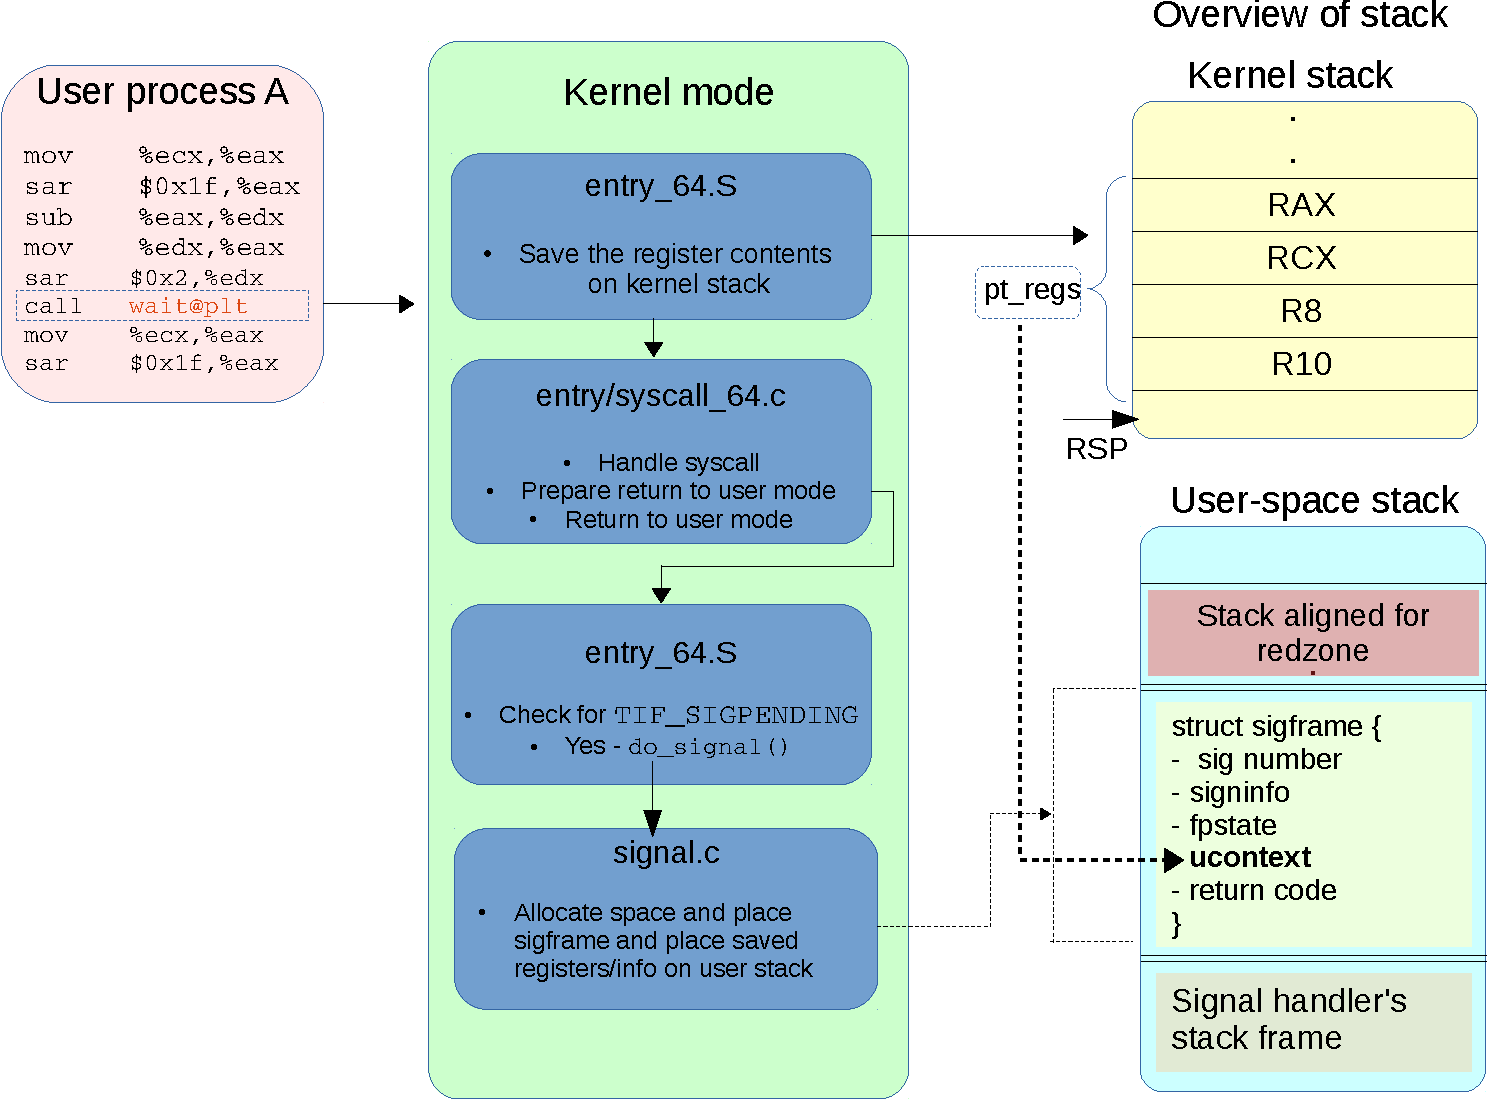
\includegraphics[height=2.5in, width=3in]{3.pdf}
\caption{Preparing Signal Delivery}
\label{fig:sig1}
\end{figure}

\begin{figure}
\centering
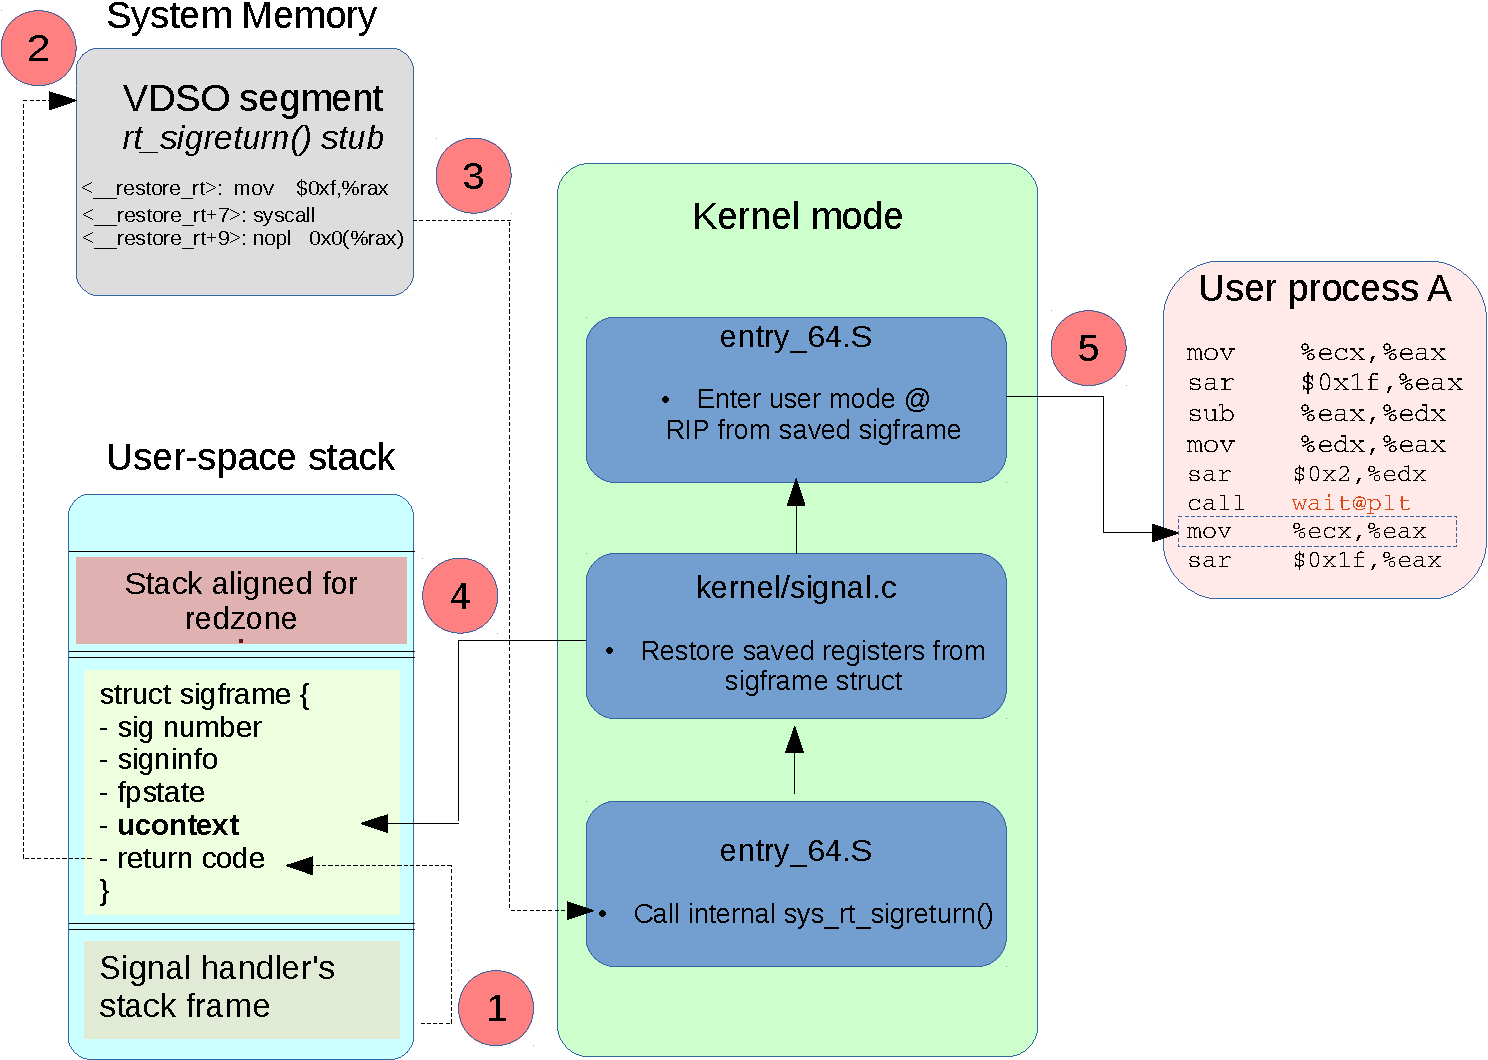
\includegraphics[height=2.5in, width=3in]{4.pdf}
\caption{Sequence of events after signal handler returns}
\label{fig:sig2}
\end{figure}

\subsection{Signal Return Oriented Programming}
Signal return oriented programming, like ROP, is a form of exploitation that utilizes assembly instructions already present in the ELF's text section, or in the dynamically loaded libraries. In a traditional ROP exploit, an attacker who has control of the stack as well as an overwritten return address can repeatedly return to a series of gadgets (assembly instructions), that do some task. That task is usually maintenance work to get specific values into registers, then a series of instructions to \textit{mmap} a region of memory with executable permissions where shell code will be copied. Lastly, an exploit, after copying shellcode into this executable memory region, would return into the shellcode to finalize the exploit.

In SROP the idea is the same, an attacker will repeatedly setup signal frames on the stack, and call the sigreturn system call. The kernel will handle moving the execution flow to the next location the attacker chooses. The exploit would be essentially the same, the attacker will try and get some memory marked executable and copy shell code into it. There are only two major difference between ROP and SROP. The first being how control flow is modified, ROP through returns, SROP through the kernel. Lastly, and probably the most important, ROP requires a significant amount of maintenance before the real guts of the exploit are run (returning to the shell code). The maintenance, getting registers with specific values, is required because the system calls require specific parameters to be passed, so the correct parameters must be in the correct registers in order for the exploit to continue. If there are no such assembly instructions in the shared library or ELF section of the program, then the attacker has no way to setup the necessary registers with the correct values, and the exploit has failed. With SROP, however, this entire maintenance part of the attack is eliminated. Because the signal frame was supposed to only be used when the kernel delivered a signal, it contains all the saved registers of the program. Those saved registers will be restored once the program calls sigreturn. Now an attacker who used to have to look for a series of gadgets, to return to, possibly thousands of gadgets to chain together, now simply has to do one sigreturn and all the registers are set in a manner that they require for their exploit.

\section {System Implementation}
We classify the system implementation in two sections - construction
of the exploit and the kernel implementation to mitigate the exploitation.

\subsection{A simple SROP exploit}
We implemented an exploit by carefully constructing a stack frame to give
control to a shellcode. The key idea in creating this exploit is to make
the instruction pointer (IP) point to the code that we want to execute. 
Unlike return oriented programming, SROP needs to know the location of 
code that executes a sigreturn system call. To accomplish this, we simply
created a gadget function that respects the system ABI to execute a system
call. Essentially, the gadget sets the system register RAX with the syscall
number (0x15 for sigreturn) and calls syscall instruction to execute sigreturn.
See Figure~\ref{fig:SFEC} for more details.

\subsubsection{Finding gadgets}
\par The ideal way of constructing an attack is to find an address of a
syscall instruction in the system address map. Although the vsyscall area provides 
an address of a syscall instruction, on 64 bit kernels the area is emulated. 
The kernel has a mechanism to check if the syscall number was the one which the 
vsycall area supports to execute, if not, the kernel throws a SIGSEV error 
saying an exploit has been attempted.  
\par So, in order to get the exploit working, we placed a gadget with a syscall 
instruction and have the code point to this gadget instead of the vsyscall area.
Although there are other methods to find the syscall address, such as finding a 
syscall address in libc shared library, this method is more elegant and simple to 
construct the attack.

\subsubsection{Preparing arbitrary code execution}
In order to execute the shellcode, we first need to ensure that sigreturn system
call executes successfully so that it restores the shellcode context later on. We
place a fake ucontext frame on stack such that it executes a execve instruction to
load shell. For this purpose, it is important to set the code segment register to 
point to 0x33 so that it runs in 64 bit mode, RAX set to syscall number of execve
system call, RDI and RSI points to the arguments (shell in our case) respectively.
When the executable is loaded, it overwrites the return address with the sigreturn
system call address and loads the fake ucontext frame to launch the shell.

\begin{figure}
\centering
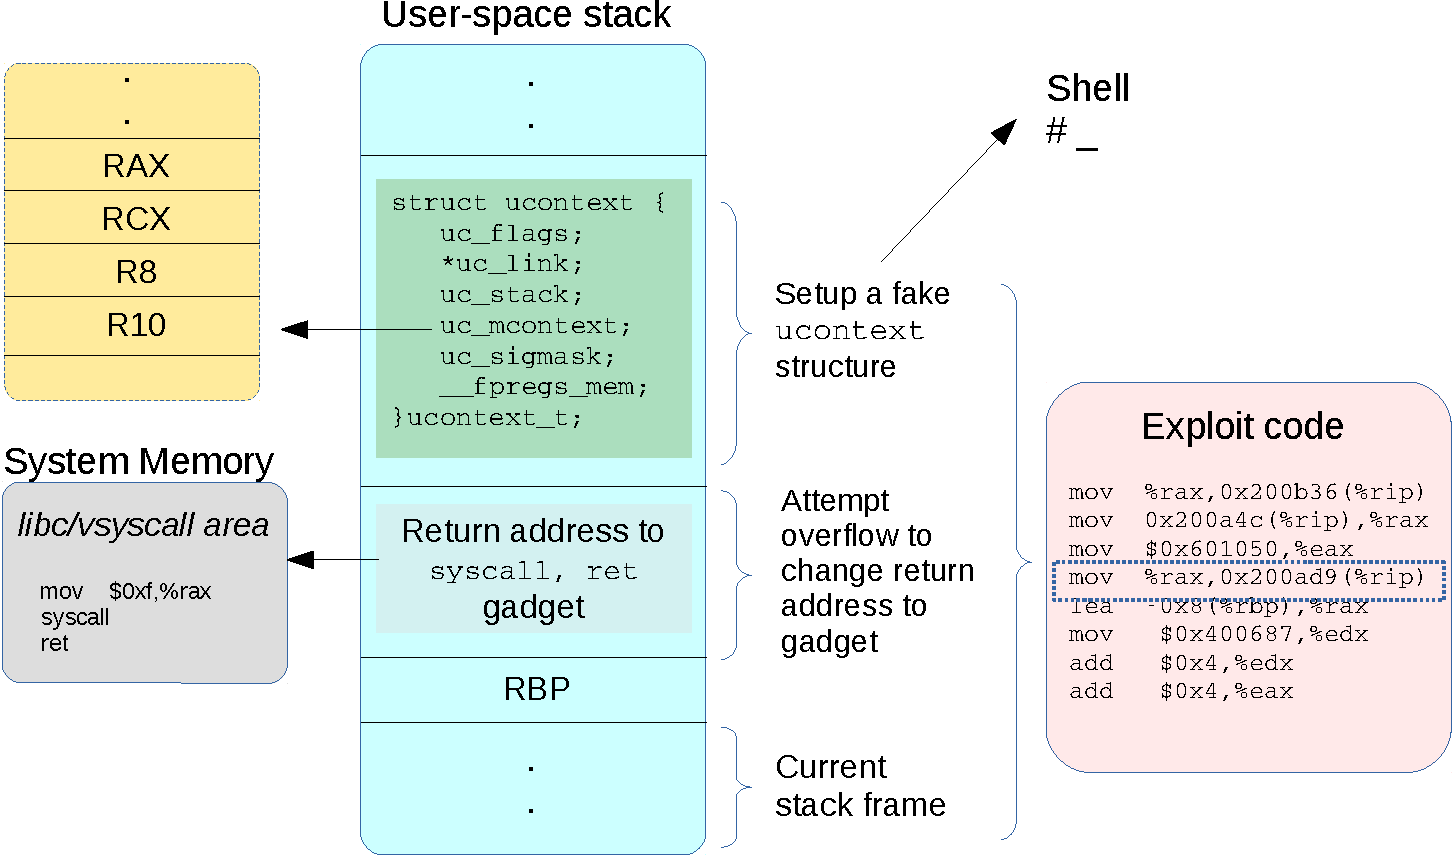
\includegraphics[height=2.5in, width=3in]{5.pdf}
\caption{Stack frame of exploit code}
\label{fig:SFEC}
\end{figure}

\subsection{Mitigating SROP}
To mitigate SROP exploits we need the kernel to remember or have the ability to derive whether or not the signal frame placed on the user stack is legitimate. A legitimate signal frame is a frame that was placed on the stack, by the kernel, during the delivery of a pending signal. If the kernel can determine the legitimacy of a signal frame it can then also detect signal frames that are apart of a SROP exploit, or buggy program. To give the kernel the ability to detect legitimate signal frames we place a cookie within the signal frame that will be audited during the \textit{sigreturn} system call. If there is no cookie in the frame, or the cookie in the frame doesn't match what the kernel expects, the process is gracefully terminated with a SIGSEV, more commonly known as a segmentation fault. 
\subsubsection{Design Choices}
There are a series of design choices we have to make in order to build a defense mechanism that is fast, secure and most important to us, could be accepted by the upstream kernel developers. The decision to use a cookie within the signal frame comes from the stack buffer overflow mechanism in StackGuard. A cookie in the signal frame increases the length of the frame only by 8 bytes, a small price to pay for protections against an exploitation method. To verify the cookie during a \textit{sigreturn} system call we need to remember the cookies we've placed in the frame. One idea is to save every cookie in a list on the process' local storage struct. This method fails for multiple reasons. First being an attacker could send many signals to a process causing the list to get filled up with cookies, after a certian time the range of cookies in the list is very large, possibly allowing an attacker to guess a correct cookie in the list. The second reason this fails is in implementation details. In order to save the cookies in this mechanism the kernel would have to allocate memory for nodes in the linked list on the signal-fast path. More over, on the sigreturn path the kernel would have to walk a linked list, possibly quite large, searching for the cookie. Due to these implementation issues saving every cookie was quickly excluded. Another approach we designed, but quickly shot down, was to hash the entire signal frame and save the hash at the bottom of the signal frame. We quickly realized an attacker could hash their custom signal frame, place the hash at the bottom, thus tricking the kernel. We decided the following goals had to be met:\\
\begin{itemize}
  \item The kernel shouldn't have to remember every cookie it puts in a signal frame.
  \item The signal delivery code, and sigreturn code needs to remain fast.
  \item The only location the cookie should be saved is on the process' stack.
  \item The cookie should not be the same for every signal, even within the same process.
\end{itemize}
%To mitigate SROP the kernel needs to remember during signal delivery that a signal was sent to the userland process. That way during the \textit{sigreturn} systemcall the kernel can verify that it is actually handling the cleanup of a signal it sent. %

\begin{figure}
\centering
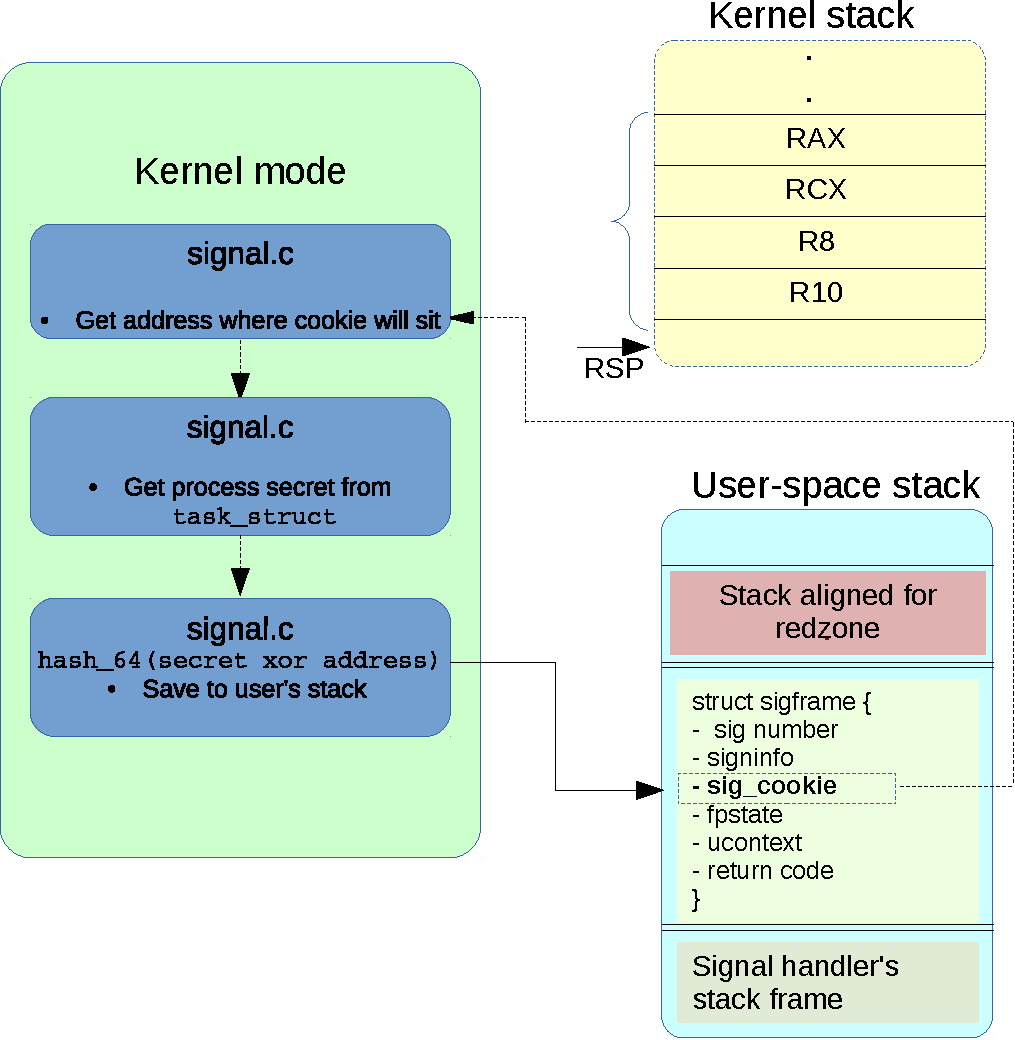
\includegraphics[height=2.7in, width=2.5in]{6.pdf}
\caption{Storing \texttt{sig\_cookie}on user-space stack}
\label{fig:sig6}
\end{figure}

\begin{figure}
\centering
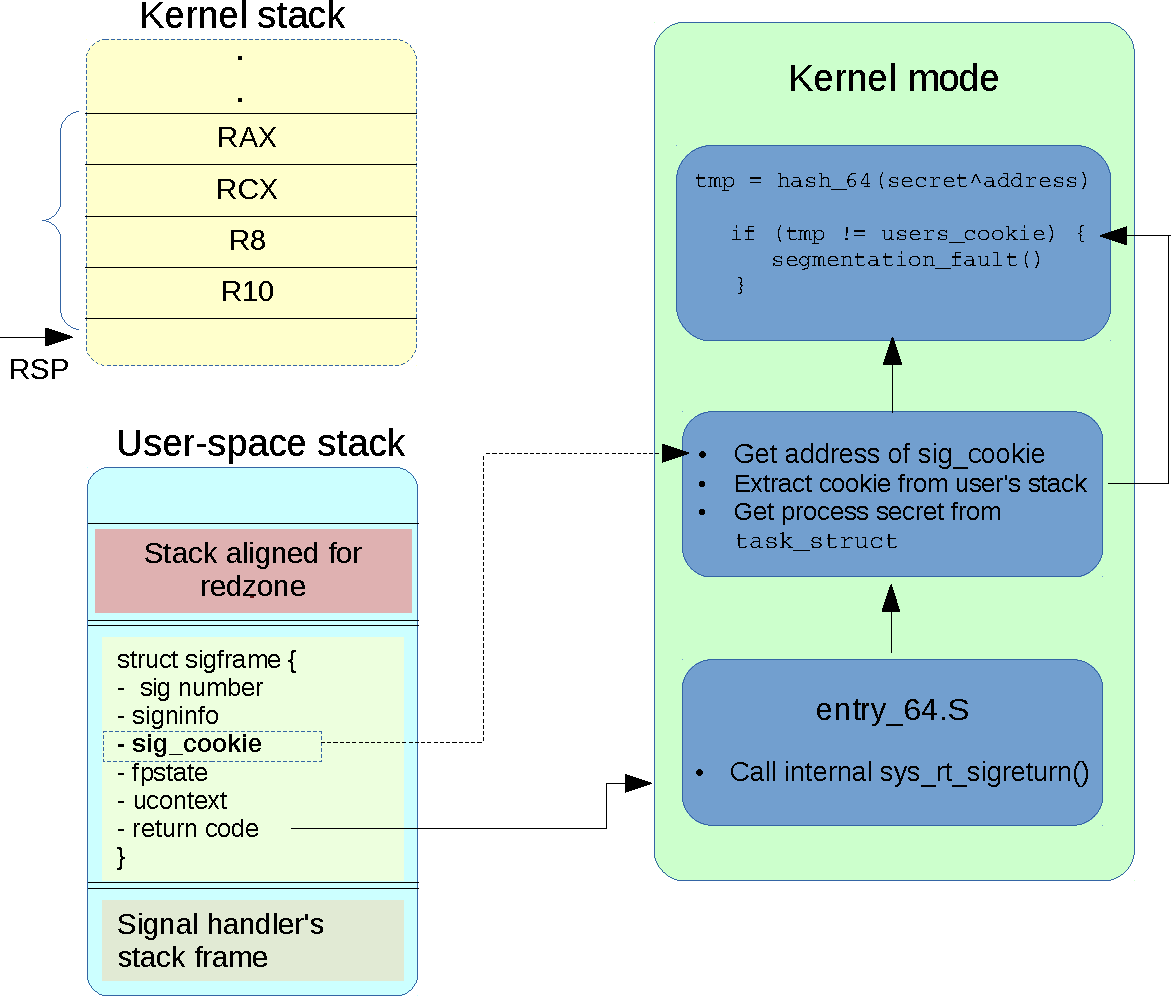
\includegraphics[height=2.7in, width=2.7in]{7.pdf}
\caption{Verfication of \texttt{sig\_cookie} on sigreturn}
\label{fig:sig7}
\end{figure}

\subsubsection{Implementation}
To realize the goals outlined in the previous section we came up with the following implementation. Each process will generate a 64 bit secret during start up, the secret will be held in the process' control block. During delivery of a signal, the kernel will generate a cookie based on the 64 bit secret as well as the address, in user-land, of where the cookie will be stored. From there the kernel places the cookie at the address and continues with normal signal delivery. Upon execution of a \textit{sigreturn} system call, the kernel extracts the cookie from the frame, it then does the same calculation as above. If the calculated and extracted cookie differ then either the process broke the ABI by moving the signal frame, or there was an exploitation attempt. This implementation meets all the goals we outlined in the previous section. The kernel doesn't have to remember every cookie it places in a frame, it only has to remember a secret once. The signal delivery and signal return code remain fast, no memory allocations or costly list walks occur. The cookie changes for each signal due to the fact we use the memory address of where the cookie is to be stored in the actual cookie calculation. Figures~\ref{fig:sig6} and ~\ref{fig:sig7} depict the same explained above.
\\
\indent
We implemented this protection mechanism on top of the 4.1 Linux tree, we selected 4.1 instead of mainline due to mainline not running correctly in our Xen virtual machine. We generate the cookie using the following code:
\\
\begin{verbatim}
/* Take address of sig cookie, xor with secret */
temp = &frame->sig_cookie ^ current->sigret_secret

/* hash the cookie */
sig_cookie = hash_64(temp);

/* place the hashed cookie on the users stack */
__put_user(temp, &frame->sig_cookie);

\end{verbatim}

To verify the cookie we do the following:

\begin{verbatim}

hashed_cookie;

__get_user(&hashed_cookie, &frame->sig_cookie);

/* do the same calculation as above */

...

if (hashed_cookie != calculated_cookie)
   send_SIGSEV();

....

\end{verbatim}

\section{Results}
We tested our implementation in two ways. First does the kernel boot and can you run a normal distribution below the modified kernel? Second, does it actually stop SROP exploits?

To answer the first question we implemented our changes in our 4.1 Linux kernel, then installed the kernel on top of a 14.03 Ubuntu distribution. From there we used the Operating system for our day-to-day tasks like browsing the web, checking mail, not doing home work, etc. During this time we saved the kernel log, which logs a multitude of things, and later parsed it for two things, segmentation faults, and SROP detection errors. The reason behind looking for both of these error messages is two-fold. For segmentation faults we wanted to make sure first that this new implementaiton didnt break any sort of application that was working outside of the kernel ABI. An example would be an application using hard-coded values in a signal handler function to pull some information out of the signal frame. Since we added a new cookie to the frame, these hard-coded values would be incorrect. Secondly for SROP errors, we wanted to make sure that no applications were falsely triggering the mitigation check. We were pleased to see that during our 8 hour run on the virtual machine, no processes crashed and our mitigation did not have any false positives.

Lastly, we ran two exploits on the new protected operating system. A simple dummy exploit, which calls a sigreturn with a fake signal stack, and a vulnerable echo server. For the dummy exploit, all we had to do was compile and run it. When we run the exploit the kernel correctly detects that a fake frame was used and terminates the application. In the kernel log we can see the kernel log \textit{Signal cookies do not match! Possible exploit attempt!,}. Lastly, we tested the vulnerable server, which contains a buffer overflow vulnerability. We launch the server, and from another machine start our exploit, which utilizes the SROP vector. Once the control flow has been hi-jacked and a sigreturn is called, the kernel detects a SROP attack, logs the message above and terminates the server with a SIGSEV, or segmentation fault.

We plan to clean up the kernel implementation a tiny bit and submit the code up-stream to the \textit{kernel hardening} mailing list, which deals with protecting user-space and the Linux kernel from attack vectors like ROP, return-to-userland, etc. We believe the patch after an iteration or two will be featured in one of the upcoming Linux kernels.

\section{Related Work}
For this work, \cite{bosman2014framing} is most relevant and a one 
stop reference. The paper provides detailed technical information 
on signal handling on UNIX based systems and introduces SROP as a 
generic exploitation technique. It also points to hints on abusing 
sigreturn system call, backdoor techniques based on SROP and ways to 
mitigate SROP attacks. 

\par In our current work, we have implemented a simple execve based 
exploit technique and a stack cookie based kernel level implementation
to address the exploitation as suggested in the paper. The paper authors
have also submitted a kernel patch targeting a different approach - counter
per process in the kernel space that keeps track of number of signal handlers
currently executing, the counter increases on signal delivery and decreases
on sigreturn path. Although this technique prevents SROP technique, it has
its own drawbacks in terms of counter roll-over and creates complications with
multi-threaded applications. We presume that these are some valid reasons why
the patch has not made it into the mainline kernel. In contrast, our approach 
is more elegant and leaves less to no room for the attacker to guess the cookie
value. Moreover, techniques suggested in the paper target older kernel versions, 
we have tested the exploit and the kernel fix on the latest kernel version (4.3).

\par As SROP is a type of an ROP attack, we find \cite{cowan1998stackguard}
related as this work implements a compiler feature which adds a cookie to the stack, 
as well as support to verify the cookie upon return of a function.  Buffer overflow 
attacks are probably the most famous form of attack gaining notoriety in the early 90's
The method works by modifying gcc such that it generates code that places a
32 bit identifier on the stack before the return address during a call instruction.
Also prior to a return gcc has the function call a verify method which validates 
that the 32 bit identifier is the same identifier that was placed there previously.
This research is very similar to the approach we have taken to prevent SROP.  
We utilize a stack cookie generated by the kernel to prevent an attacker from 
creating an arbitrary signal frame on the stack causing the kernel to jump arbitrarily 
through the code.

\par Another relevant reference is \cite{li2010defeating} as the work implements a 
compiler technique to prevent ret instructions from being generated in a kernel image. 
By removing ret instructions from the kernel it prevents an entire class of attack, 
Return Oriented Programming (ROP) from ever occurring because the fundamental feature 
of the attack is removed. The authors modify LLVM such that it will never generate a ret 
op-code, as well as will never generate a sequence of instructions that contain a ret op-code, 
if you were to jump between instructions. Instead of developing a technique to systematically 
remove the necessary elements for the attack we have used a hardening technique to 
prevent the attack.

\bibliographystyle{abbrv}
\bibliography{sigproc}
\end{document}
